\section{Program Analysis}
\enumstart
	\item Can automatically learn facts about a program
	\\ 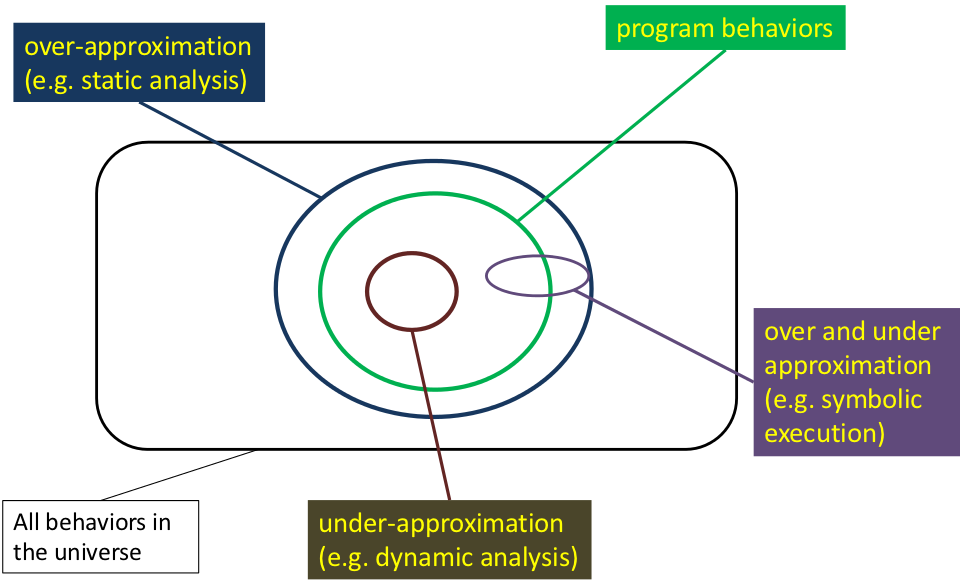
\includegraphics[width=0.5\textwidth]{img/program_analysis.png}
\enumend

\subsection{Static program analysis}
\enumstart
	\item We use abstract interpretation $\rightarrow$ a general theory of how to do approximation systematically
\enumend

\subsection{Abstract interpretation}
\enumstart
	\item Step-by-step
	\enumstart
		\item Select/define an abstract domain (depends on what you want to prove)
		\item Define abstract semantics for the language w.r.t. the domain
		\enumstart
			\item Prove sound w.r.t. concrete semantics
			\item Involves defining abstract transformers
		\enumend
		\item Iterate abstract transformers over the abstract domain $\rightarrow$ until fixpoint is reached
	\enumend
	\item The fixpoint is the over-approximation of the program
\enumend

\subsection{Abstract transformer}
\enumstart
	\item Effect of statement and expression evaluation on an abstract state
	\item Defined per programming language once and for all
	\item Abstract transformers define the abstract semantics of the language
	\item Correctness(soundness): produces a superset of what a concrete transformer would produce
	\item Precision: the set produced by the abstract transformer is as small as possible
	\item Goal, be perfectly sound and as precise as possible
	\item Sometimes, computing the most precise transformer (best transformer) is not possible
\enumend

\subsection{Iterate abstract transformers}
\enumstart
	\item Start with the least abstract element for all program-counter values
	\item Iterate the different statements/expressions and apply abstract transformers.
	\item Whenever we have two abstract elements $A$ and $B$, we can join them to produce their (least) upper bound (denoted by $A \sqcup B$)
	\item $A \sqsubseteq (A \sqcup B)$ and $B \sqsubseteq (A \sqcup B)$
	\item $D \sqsubseteq E$ means that $E$ is more abstract than $D$
	\item If it never terminates, do widening
\enumend

\subsection{Widening}
\enumstart
	\item Ensures termination at the expense of precision
	\item Do instead of join, whenever you like
\enumend
